\documentclass[tikz,border=10pt]{standalone}

\usepackage{tikz}
\usepackage{lmodern}

\begin{document}
% Vector plot of the recorded Tahoe estimator fit times (seconds).
% Columns: samples(M), TorchDR 1/2/4/8 GPUs, cuML 1 GPU, umap-learn 64 cores.
% 1, 6.08, 5.52, 6.88, 17.34, 22.56, 64.32
% 5, 26.06, 16.42, 13.08, 21.18, 71.19, 290.44
% 10, 88.69, 50.76, 32.86, 34.68, 157.76, 643.22
% 20, 190.69, 108.51, 70.37, 60.77, 241.19, NA
% 40, 385.59, 283.13, 182.46, 142.8, 391.04, NA
% 80, NA, NA, NA, 379.9, 719.37, NA
% The cuML 80M measurement is not displayed in this figure.
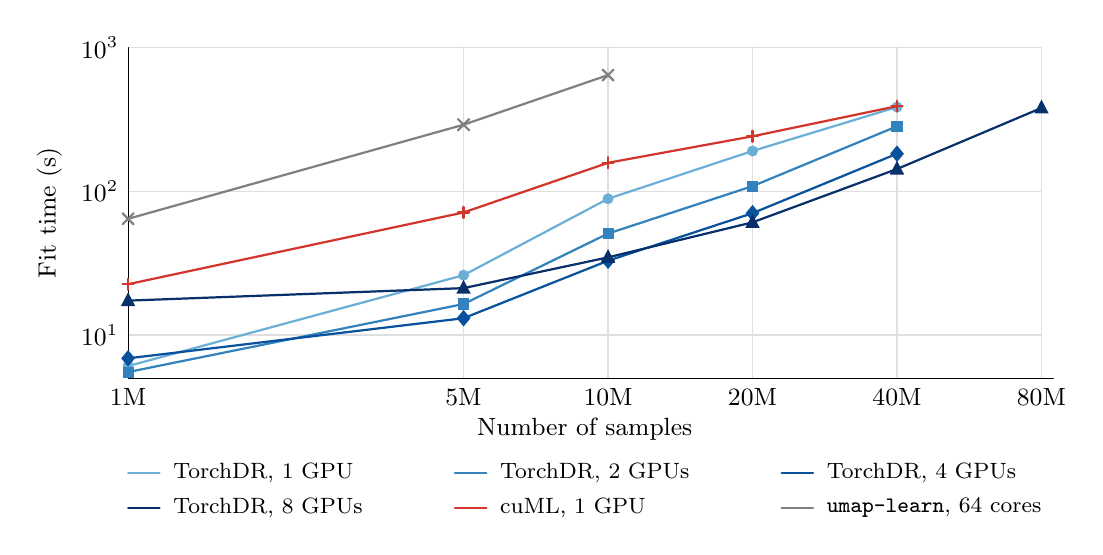
\begin{tikzpicture}[font=\small,line cap=round]
\definecolor{tdone}{HTML}{6BAED6}
\definecolor{tdtwo}{HTML}{3182BD}
\definecolor{tdfour}{HTML}{08519C}
\definecolor{tdeight}{HTML}{08306B}
\definecolor{cumlred}{HTML}{D1352C}
\draw[gray!25] (0,0) -- (0,4.2);
\node[below] at (0,0) {1M};
\draw[gray!25] (4.260466980394103,0) -- (4.260466980394103,4.2);
\node[below] at (4.260466980394103,0) {5M};
\draw[gray!25] (6.095350235295578,0) -- (6.095350235295578,4.2);
\node[below] at (6.095350235295578,0) {10M};
\draw[gray!25] (7.930233490197052,0) -- (7.930233490197052,4.2);
\node[below] at (7.930233490197052,0) {20M};
\draw[gray!25] (9.765116745098526,0) -- (9.765116745098526,4.2);
\node[below] at (9.765116745098526,0) {40M};
\draw[gray!25] (11.6,0) -- (11.6,4.2);
\node[below] at (11.6,0) {80M};
\draw[gray!25] (0,0.5494608867208136) -- (11.6,0.5494608867208136);
\node[left] at (0,0.5494608867208136) {$10^{1}$};
\draw[gray!25] (0,2.374730443360407) -- (11.6,2.374730443360407);
\node[left] at (0,2.374730443360407) {$10^{2}$};
\draw[gray!25] (0,4.2) -- (11.6,4.2);
\node[left] at (0,4.2) {$10^{3}$};
\draw (0,4.2) -- (0,0) -- (11.75,0);
\node[rotate=90] at (-1.0,2.1) {Fit time (s)};
\node at (5.8,-0.65) {Number of samples};
\draw[tdone,thick] plot coordinates {(0.00000,0.15503) (4.26047,1.30873) (6.09535,2.27959) (7.93023,2.88640) (9.76512,3.44457)};
\begin{scope}[shift={(0.00000,0.15503)}]
\fill[tdone] (0,0) circle (2pt);
\end{scope}
\begin{scope}[shift={(4.26047,1.30873)}]
\fill[tdone] (0,0) circle (2pt);
\end{scope}
\begin{scope}[shift={(6.09535,2.27959)}]
\fill[tdone] (0,0) circle (2pt);
\end{scope}
\begin{scope}[shift={(7.93023,2.88640)}]
\fill[tdone] (0,0) circle (2pt);
\end{scope}
\begin{scope}[shift={(9.76512,3.44457)}]
\fill[tdone] (0,0) circle (2pt);
\end{scope}
\draw[tdone,thick] (0,-1.2) -- (0.4,-1.2);
\node[right,font=\footnotesize] at (0.45,-1.2) {TorchDR, 1 GPU};
\draw[tdtwo,thick] plot coordinates {(0.00000,0.07843) (4.26047,0.94257) (6.09535,1.83723) (7.93023,2.43947) (9.76512,3.19973)};
\begin{scope}[shift={(0.00000,0.07843)}]
\fill[tdtwo] (-2pt,-2pt) rectangle (2pt,2pt);
\end{scope}
\begin{scope}[shift={(4.26047,0.94257)}]
\fill[tdtwo] (-2pt,-2pt) rectangle (2pt,2pt);
\end{scope}
\begin{scope}[shift={(6.09535,1.83723)}]
\fill[tdtwo] (-2pt,-2pt) rectangle (2pt,2pt);
\end{scope}
\begin{scope}[shift={(7.93023,2.43947)}]
\fill[tdtwo] (-2pt,-2pt) rectangle (2pt,2pt);
\end{scope}
\begin{scope}[shift={(9.76512,3.19973)}]
\fill[tdtwo] (-2pt,-2pt) rectangle (2pt,2pt);
\end{scope}
\draw[tdtwo,thick] (4.15,-1.2) -- (4.550000000000001,-1.2);
\node[right,font=\footnotesize] at (4.6000000000000005,-1.2) {TorchDR, 2 GPUs};
\draw[tdfour,thick] plot coordinates {(0.00000,0.25302) (4.26047,0.76230) (6.09535,1.49252) (7.93023,2.09617) (9.76512,2.85143)};
\begin{scope}[shift={(0.00000,0.25302)}]
\fill[tdfour] (0,3pt)--(2.5pt,0)--(0,-3pt)--(-2.5pt,0)--cycle;
\end{scope}
\begin{scope}[shift={(4.26047,0.76230)}]
\fill[tdfour] (0,3pt)--(2.5pt,0)--(0,-3pt)--(-2.5pt,0)--cycle;
\end{scope}
\begin{scope}[shift={(6.09535,1.49252)}]
\fill[tdfour] (0,3pt)--(2.5pt,0)--(0,-3pt)--(-2.5pt,0)--cycle;
\end{scope}
\begin{scope}[shift={(7.93023,2.09617)}]
\fill[tdfour] (0,3pt)--(2.5pt,0)--(0,-3pt)--(-2.5pt,0)--cycle;
\end{scope}
\begin{scope}[shift={(9.76512,2.85143)}]
\fill[tdfour] (0,3pt)--(2.5pt,0)--(0,-3pt)--(-2.5pt,0)--cycle;
\end{scope}
\draw[tdfour,thick] (8.3,-1.2) -- (8.700000000000001,-1.2);
\node[right,font=\footnotesize] at (8.75,-1.2) {TorchDR, 4 GPUs};
\draw[tdeight,thick] plot coordinates {(0.00000,0.98579) (4.26047,1.14436) (6.09535,1.53525) (7.93023,1.97990) (9.76512,2.65715)};
\begin{scope}[shift={(0.00000,0.98579)}]
\fill[tdeight] (0,3pt)--(-2.6pt,-2pt)--(2.6pt,-2pt)--cycle;
\end{scope}
\begin{scope}[shift={(4.26047,1.14436)}]
\fill[tdeight] (0,3pt)--(-2.6pt,-2pt)--(2.6pt,-2pt)--cycle;
\end{scope}
\begin{scope}[shift={(6.09535,1.53525)}]
\fill[tdeight] (0,3pt)--(-2.6pt,-2pt)--(2.6pt,-2pt)--cycle;
\end{scope}
\begin{scope}[shift={(7.93023,1.97990)}]
\fill[tdeight] (0,3pt)--(-2.6pt,-2pt)--(2.6pt,-2pt)--cycle;
\end{scope}
\begin{scope}[shift={(9.76512,2.65715)}]
\fill[tdeight] (0,3pt)--(-2.6pt,-2pt)--(2.6pt,-2pt)--cycle;
\end{scope}
\draw[tdeight,thick] (0,-1.65) -- (0.4,-1.65);
\node[right,font=\footnotesize] at (0.45,-1.65) {TorchDR, 8 GPUs};
\draw[cumlred,thick] plot coordinates {(0.00000,1.19440) (4.26047,2.10536) (6.09535,2.73613) (7.93023,3.07264) (9.76512,3.45569)};
\begin{scope}[shift={(0.00000,1.19440)}]
\draw[cumlred,thick] (-2pt,0)--(2pt,0) (0,-2pt)--(0,2pt);
\end{scope}
\begin{scope}[shift={(4.26047,2.10536)}]
\draw[cumlred,thick] (-2pt,0)--(2pt,0) (0,-2pt)--(0,2pt);
\end{scope}
\begin{scope}[shift={(6.09535,2.73613)}]
\draw[cumlred,thick] (-2pt,0)--(2pt,0) (0,-2pt)--(0,2pt);
\end{scope}
\begin{scope}[shift={(7.93023,3.07264)}]
\draw[cumlred,thick] (-2pt,0)--(2pt,0) (0,-2pt)--(0,2pt);
\end{scope}
\begin{scope}[shift={(9.76512,3.45569)}]
\draw[cumlred,thick] (-2pt,0)--(2pt,0) (0,-2pt)--(0,2pt);
\end{scope}
\draw[cumlred,thick] (4.15,-1.65) -- (4.550000000000001,-1.65);
\node[right,font=\footnotesize] at (4.6000000000000005,-1.65) {cuML, 1 GPU};
\draw[gray,thick] plot coordinates {(0.00000,2.02491) (4.26047,3.21993) (6.09535,3.85020)};
\begin{scope}[shift={(0.00000,2.02491)}]
\draw[gray,thick] (-2pt,-2pt)--(2pt,2pt) (-2pt,2pt)--(2pt,-2pt);
\end{scope}
\begin{scope}[shift={(4.26047,3.21993)}]
\draw[gray,thick] (-2pt,-2pt)--(2pt,2pt) (-2pt,2pt)--(2pt,-2pt);
\end{scope}
\begin{scope}[shift={(6.09535,3.85020)}]
\draw[gray,thick] (-2pt,-2pt)--(2pt,2pt) (-2pt,2pt)--(2pt,-2pt);
\end{scope}
\draw[gray,thick] (8.3,-1.65) -- (8.700000000000001,-1.65);
\node[right,font=\footnotesize] at (8.75,-1.65) {\texttt{umap-learn}, 64 cores};
\draw[tdeight,thick] (9.76512,2.65715) -- (11.60000,3.43278);
\begin{scope}[shift={(11.60000,3.43278)}]
\fill[tdeight] (0,3pt)--(-2.6pt,-2pt)--(2.6pt,-2pt)--cycle;
\end{scope}
\end{tikzpicture}
\end{document}
